% Options for packages loaded elsewhere
\PassOptionsToPackage{unicode}{hyperref}
\PassOptionsToPackage{hyphens}{url}
%
\documentclass[
]{book}
\usepackage{amsmath,amssymb}
\usepackage{lmodern}
\usepackage{ifxetex,ifluatex}
\ifnum 0\ifxetex 1\fi\ifluatex 1\fi=0 % if pdftex
  \usepackage[T1]{fontenc}
  \usepackage[utf8]{inputenc}
  \usepackage{textcomp} % provide euro and other symbols
\else % if luatex or xetex
  \usepackage{unicode-math}
  \defaultfontfeatures{Scale=MatchLowercase}
  \defaultfontfeatures[\rmfamily]{Ligatures=TeX,Scale=1}
\fi
% Use upquote if available, for straight quotes in verbatim environments
\IfFileExists{upquote.sty}{\usepackage{upquote}}{}
\IfFileExists{microtype.sty}{% use microtype if available
  \usepackage[]{microtype}
  \UseMicrotypeSet[protrusion]{basicmath} % disable protrusion for tt fonts
}{}
\makeatletter
\@ifundefined{KOMAClassName}{% if non-KOMA class
  \IfFileExists{parskip.sty}{%
    \usepackage{parskip}
  }{% else
    \setlength{\parindent}{0pt}
    \setlength{\parskip}{6pt plus 2pt minus 1pt}}
}{% if KOMA class
  \KOMAoptions{parskip=half}}
\makeatother
\usepackage{xcolor}
\IfFileExists{xurl.sty}{\usepackage{xurl}}{} % add URL line breaks if available
\IfFileExists{bookmark.sty}{\usepackage{bookmark}}{\usepackage{hyperref}}
\hypersetup{
  pdftitle={Application for the International Digital Development Traineeship in Digital Banking},
  hidelinks,
  pdfcreator={LaTeX via pandoc}}
\urlstyle{same} % disable monospaced font for URLs
\usepackage{longtable,booktabs,array}
\usepackage{calc} % for calculating minipage widths
% Correct order of tables after \paragraph or \subparagraph
\usepackage{etoolbox}
\makeatletter
\patchcmd\longtable{\par}{\if@noskipsec\mbox{}\fi\par}{}{}
\makeatother
% Allow footnotes in longtable head/foot
\IfFileExists{footnotehyper.sty}{\usepackage{footnotehyper}}{\usepackage{footnote}}
\makesavenoteenv{longtable}
\usepackage{graphicx}
\makeatletter
\def\maxwidth{\ifdim\Gin@nat@width>\linewidth\linewidth\else\Gin@nat@width\fi}
\def\maxheight{\ifdim\Gin@nat@height>\textheight\textheight\else\Gin@nat@height\fi}
\makeatother
% Scale images if necessary, so that they will not overflow the page
% margins by default, and it is still possible to overwrite the defaults
% using explicit options in \includegraphics[width, height, ...]{}
\setkeys{Gin}{width=\maxwidth,height=\maxheight,keepaspectratio}
% Set default figure placement to htbp
\makeatletter
\def\fps@figure{htbp}
\makeatother
\setlength{\emergencystretch}{3em} % prevent overfull lines
\providecommand{\tightlist}{%
  \setlength{\itemsep}{0pt}\setlength{\parskip}{0pt}}
\setcounter{secnumdepth}{5}
\usepackage{booktabs}
\ifluatex
  \usepackage{selnolig}  % disable illegal ligatures
\fi
\usepackage[]{natbib}
\bibliographystyle{apalike}

\title{Application for the International Digital Development Traineeship in Digital Banking}
\author{}
\date{\vspace{-2.5em}2022-03-30}

\begin{document}
\maketitle

{
\setcounter{tocdepth}{1}
\tableofcontents
}
\hypertarget{welcome}{%
\chapter{Welcome!}\label{welcome}}

\hypertarget{motivation}{%
\chapter{Motivation}\label{motivation}}

\hypertarget{cv}{%
\chapter{CV}\label{cv}}

\hypertarget{professional-experience}{%
\section{Professional Experience}\label{professional-experience}}

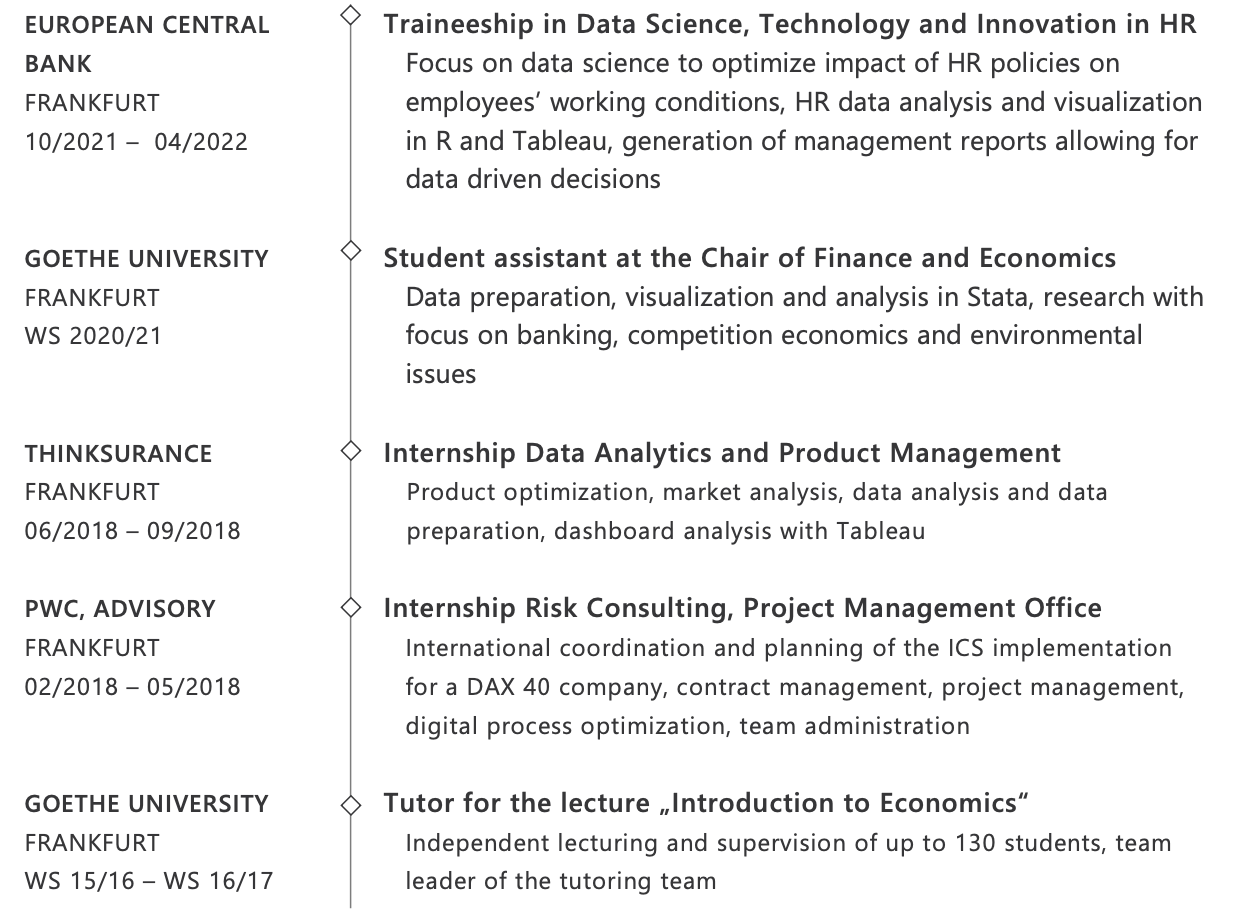
\includegraphics[width=0.85\textwidth,height=\textheight]{/Users/larazaremba/Documents/GitHub/Application/application_bookdown/_bookdown_files/Experience.png}

\hypertarget{education}{%
\section{Education}\label{education}}

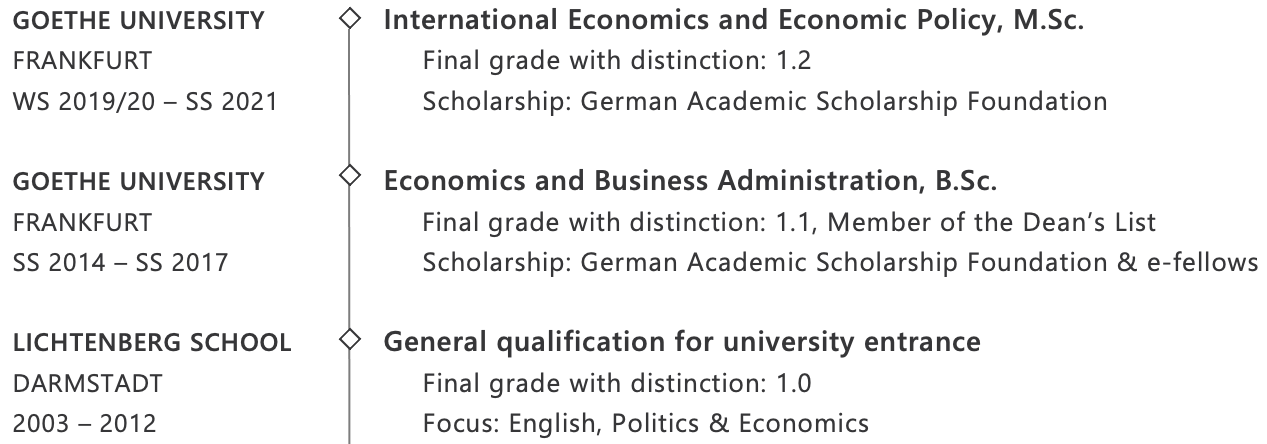
\includegraphics[width=0.85\textwidth,height=\textheight]{/Users/larazaremba/Documents/GitHub/Application/application_bookdown/_bookdown_files/Education.png}

\hypertarget{international-experience}{%
\section{International Experience}\label{international-experience}}

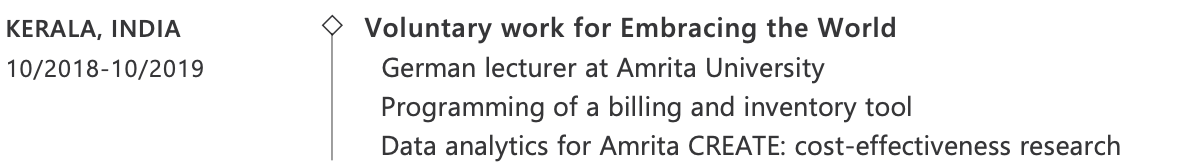
\includegraphics[width=0.82\textwidth,height=\textheight]{/Users/larazaremba/Documents/GitHub/Application/application_bookdown/_bookdown_files/International.png}

\hypertarget{voluntary-work}{%
\section{Voluntary Work}\label{voluntary-work}}

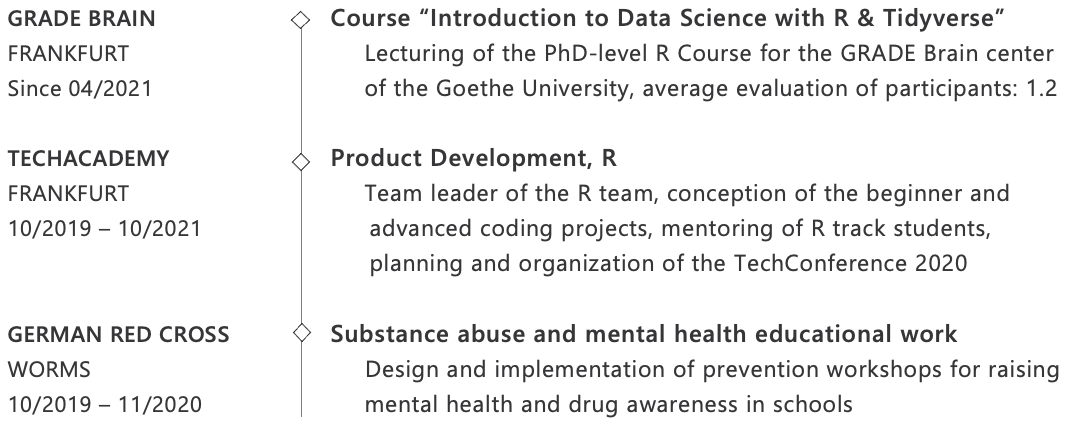
\includegraphics[width=0.82\textwidth,height=\textheight]{/Users/larazaremba/Documents/GitHub/Application/application_bookdown/_bookdown_files/Volunteer.png}

\hypertarget{skills}{%
\section{Skills}\label{skills}}

\hypertarget{it-skills}{%
\subsection{IT Skills}\label{it-skills}}

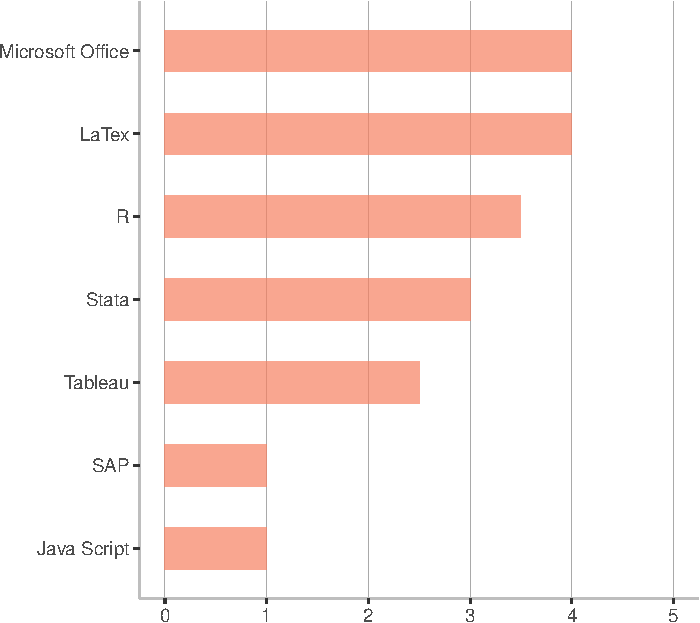
\includegraphics{application_bookdown_files/figure-latex/unnamed-chunk-1-1.pdf}

\hypertarget{languages}{%
\subsection{Languages}\label{languages}}

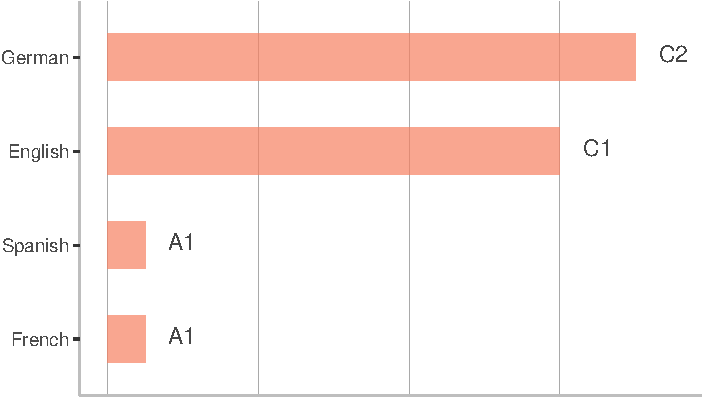
\includegraphics{application_bookdown_files/figure-latex/unnamed-chunk-2-1.pdf}

\hypertarget{info}{%
\chapter{Info}\label{info}}

\textbf{Address:}\\
Goethestrasse 31\\
64354 Reinheim

\textbf{E-mail:}\\
\href{mailto:laramariazaremba@gmail.com}{\nolinkurl{laramariazaremba@gmail.com}}

\textbf{Phone:}\\
0176/32216047

\textbf{Date of birth:}\\
12.02.1993

\textbf{Place of birth:}\\
Seeheim-Jugenheim

\textbf{Nationality:}\\
German

\hypertarget{certificates}{%
\chapter{Certificates}\label{certificates}}

\hypertarget{work}{%
\section{Work}\label{work}}

If you are interested in what previous employers had to say about me, please have a look at the following \textbf{work certificates}:

This browser does not support PDFs. Please download the \textbf{Work Certificate PDF} to view it: Download PDF.

\hypertarget{education-1}{%
\section{Education}\label{education-1}}

If you are interested in my performance in school and at university, please have a look at these \textbf{education certificates}:

This browser does not support PDFs. Please download the \textbf{Education Certificate PDF} to view it: Download PDF.

  \bibliography{book.bib,packages.bib}

\end{document}
